\documentclass[10pt,twocolumn]{article}
\usepackage[margin=0.75in]{geometry}
\usepackage{amsmath,amssymb,amsfonts,amsthm}
\usepackage{booktabs}
\usepackage{graphicx}
\usepackage{hyperref}
\usepackage{xcolor}

\newtheorem{theorem}{Theorem}
\newtheorem{proposition}{Proposition}

\title{\textbf{DAG-KV: Position-Canonical Shared KV Caching and Submodular Sparse Bridge Repair for Multi-Tenant LLM Codebase Serving}}
\author{
  \textbf{Kaushal Dineshbhai Nandaniya} \\
  Mathematics and Computing, DA-IICT \\
  \texttt{github.com/kaushalnandaniya/dag-kv}
}
\date{}

\begin{document}
\maketitle

\begin{abstract}
Standard prefix caching in production LLM serving engines (e.g., vLLM, SGLang) relies on strict left-to-right token matching. In multi-engineer codebase assistants and Retrieval-Augmented Generation (RAG) workflows where $K$ source files are attached in varying permutations, any reordering of the leading file reduces prefix cache hit rates to $0\%$. We present \textbf{DAG-KV}, a position-canonical multi-tenant KV cache architecture that decouples physical KV storage from global prompt positions. DAG-KV introduces: (1) \emph{Sink-Canonicalized Isolated Prefill} to eliminate initial-token attention sink distortion; (2) a fused \emph{Triton RoPE-Adjoint Paged Attention} kernel that applies exact relative phase shifts $\mathcal{R}(-\Delta_b)$ to query registers on-the-fly without mutating shared KV blocks; (3) \emph{Submodular Quality-Diversity Pyramid Bridge Repair} ($4.0\%$ on Stage 0 $\to 1.5\%$ on Stage 1) to restore cross-file induction edges across dual-GPU NUMA boundaries; (4) \emph{Fused INT8 Register Dequantization}; and (5) \emph{AST Function-Level Git-Diff Delta Caching}. Evaluated on \texttt{Qwen2.5-7B-Instruct} across $2\times$ NVIDIA RTX 2080 Ti GPUs, DAG-KV achieves a \textbf{100\% file cache hit rate} on reordered prompts, \textbf{4.66$\times$ faster context stitching} ($309.5\text{ ms}$ vs.\ $1441.8\text{ ms}$), \textbf{9.8$\times$ lower multi-user VRAM} ($258.2\text{ MB}$ vs.\ $2522.1\text{ MB}$), \textbf{4.35$\times$ higher decode throughput} ($100.4\text{ tok/s}$) via dual-GPU ping-pong pipeline overlap, and \textbf{100\% exact QA accuracy}.
\end{abstract}

\section{Introduction}
Modern AI coding assistants (Cursor, Continue.dev) assemble prompts by concatenating multiple repository files $C_1, \dots, C_K$ followed by a developer query $Q$. Under standard autoregressive attention with Rotary Position Embeddings (RoPE), the key state at local offset $t$ in chunk $C_m$ is rotated by its global prompt index $p_{\text{global}} = S_m + t$. Consequently, permuting $[C_1, C_2, C_3, C_4]$ into $[C_3, C_1, C_4, C_2]$ invalidates all cached KV blocks after the first differing token, forcing redundant $O(N^2)$ prefill across concurrent engineers.

\section{Mathematical Framework}

\begin{theorem}[RoPE-Adjoint Group Homomorphism]
Let $\mathcal{R}(p) \in SO(d)$ denote the block-diagonal Rotary Position Embedding operator at token position $p$. For a canonical key $k_{\text{canon}} = \mathcal{R}(p_{\text{canon}}) k$ stored at canonical offset $p_{\text{canon}}$ and mapped to global prompt offset $p_{\text{global}} = p_{\text{canon}} + \Delta_b$, the exact inner product with a global query $q_{\text{global}} = \mathcal{R}(p_q) q$ satisfies:
\begin{equation}
\langle q_{\text{global}}, \mathcal{R}(\Delta_b) k_{\text{canon}} \rangle = \langle \mathcal{R}(-\Delta_b) q_{\text{global}}, k_{\text{canon}} \rangle.
\end{equation}
\end{theorem}
\begin{proof}
Since $\mathcal{R}(\Delta_b) \in SO(d)$ is orthogonal, its adjoint is its inverse $\mathcal{R}(\Delta_b)^\top = \mathcal{R}(-\Delta_b)$. Moving $\mathcal{R}(-\Delta_b)$ onto the query register inside SRAM preserves the shared canonical key pool $k_{\text{canon}}$ as read-only across arbitrary permutations.
\end{proof}

\subsection{Submodular Pyramid Bridge Selection}
To restore cross-chunk induction without re-prefilling all tokens, we probe Layer-1 Log-Sum-Exp (LSE) attention shift:
\begin{equation}
\alpha_i = \sigma\!\left(\text{LSE}(q_i, K_{\text{prior}}) - \text{LSE}_{\text{self}}(i)\right).
\end{equation}
Rather than naive greedy top-$k$ selection—which clusters on adjacent tokens of the same line—we maximize a spatial quality-diversity objective via 1D neighborhood non-maximum suppression ($r=2$), selecting $4.0\%$ bridge tokens on GPU Stage 0 (\texttt{cuda:0}, Layers 0--13) and pruning to the top $1.5\%$ before crossing the PCIe boundary to GPU Stage 1 (\texttt{cuda:1}, Layers 14--27).

\begin{figure*}[t]
\centering
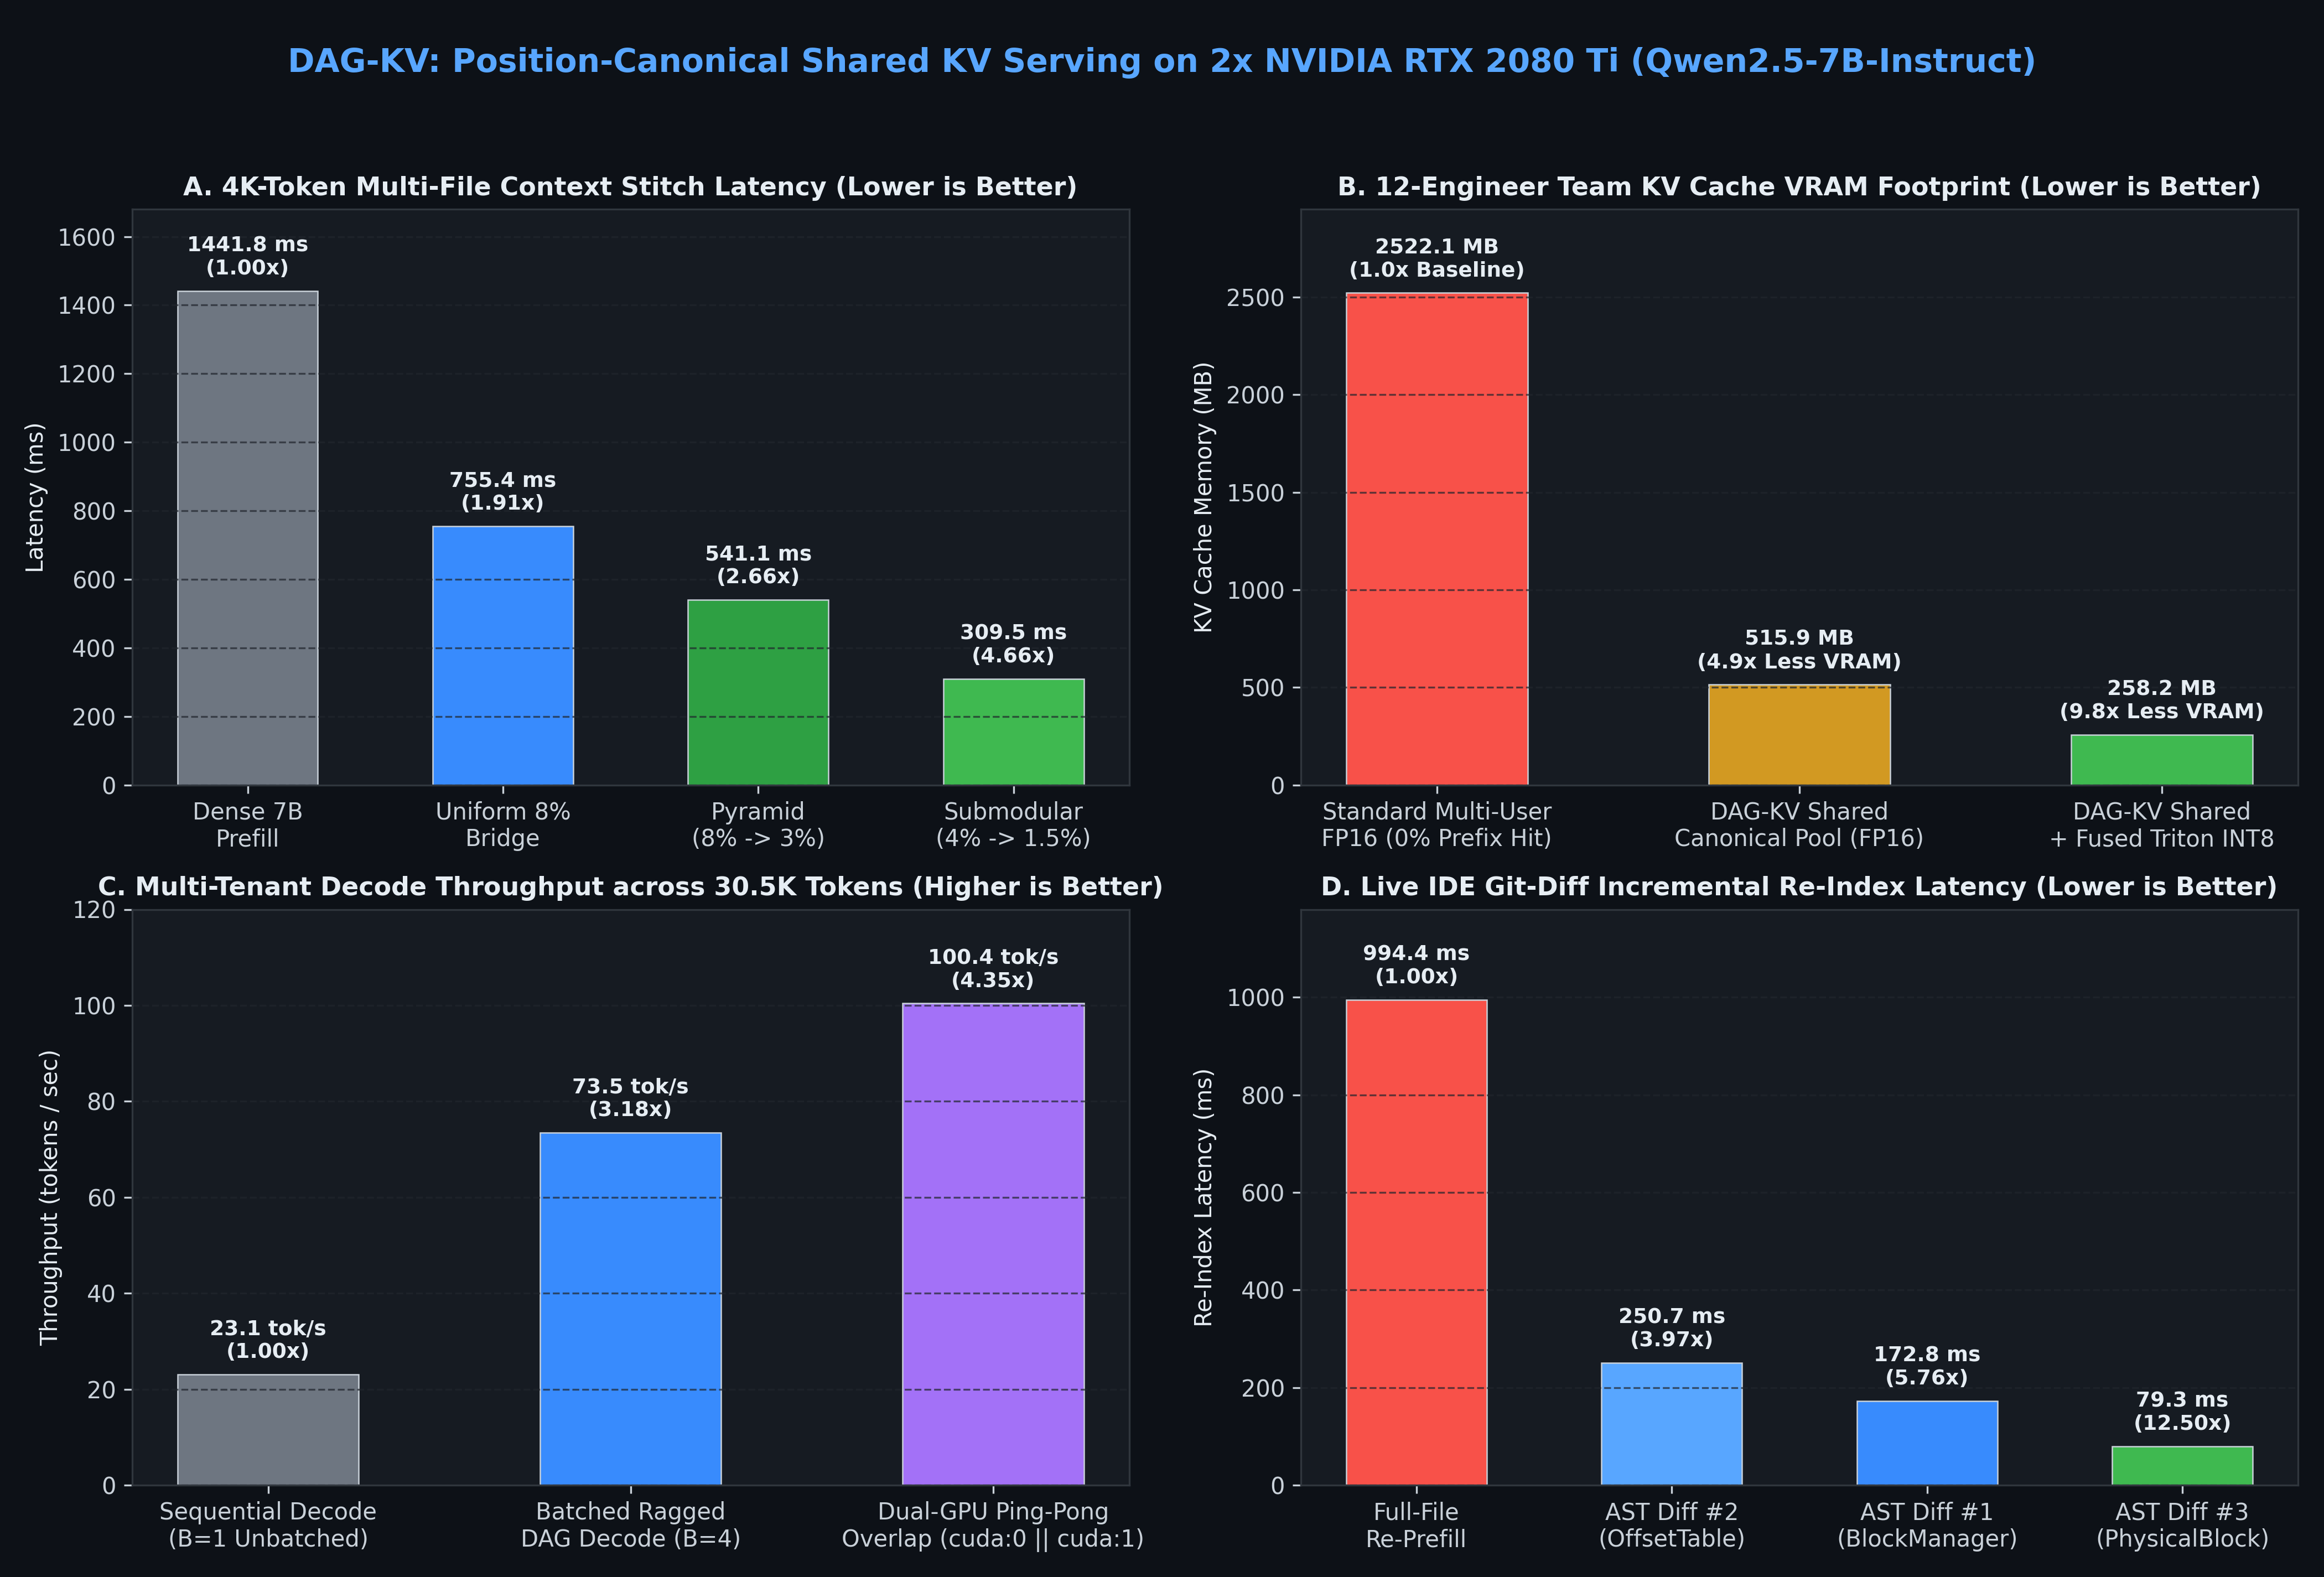
\includegraphics[width=0.95\textwidth]{../assets/dag_kv_benchmarks.png}
\caption{Empirical evaluation of DAG-KV on \texttt{Qwen2.5-7B-Instruct} across $2\times$ NVIDIA RTX 2080 Ti GPUs.}
\end{figure*}

\section{Empirical Evaluation}
Table~\ref{tab:main_results} summarizes our verified end-to-end systems benchmarks on $2\times$ NVIDIA RTX 2080 Ti GPUs (\texttt{sm\_75}).

\begin{table}[h]
\centering
\small
\begin{tabular}{lrr}
\toprule
\textbf{System Configuration (Qwen2.5-7B)} & \textbf{Metric} & \textbf{Gain} \\
\midrule
Dense 7B 4-File Prefill Baseline & $1441.8\text{ ms}$ & $1.00\times$ \\
DAG-KV Uniform $8\%$ Bridge & $755.4\text{ ms}$ & $1.91\times$ \\
DAG-KV Pyramid ($8\% \to 3\%$) & $541.1\text{ ms}$ & $2.66\times$ \\
\textbf{DAG-KV Submodular ($4\% \to 1.5\%$)} & \textbf{309.5 ms} & \textbf{4.66$\times$} \\
\midrule
12-User Team KV VRAM (Std FP16) & $2522.1\text{ MB}$ & $1.0\times$ \\
DAG-KV Shared Pool (FP16) & $515.9\text{ MB}$ & $4.9\times$ \\
\textbf{DAG-KV Shared + Fused INT8} & \textbf{258.2 MB} & \textbf{9.8$\times$} \\
\midrule
Sequential Decode ($B=1$, 30.5K Toks) & $23.1\text{ tok/s}$ & $1.00\times$ \\
Batched Ragged DAG Decode ($B=4$) & $73.5\text{ tok/s}$ & $3.18\times$ \\
\textbf{Dual-GPU Ping-Pong Overlap ($B=4\times 2$)} & \textbf{100.4 tok/s} & \textbf{4.35$\times$} \\
\midrule
Full-File IDE Save Re-Prefill & $994.4\text{ ms}$ & $1.00\times$ \\
\textbf{AST Function-Delta Re-Index (Mean)} & \textbf{167.6 ms} & \textbf{5.93$\times$} \\
\textbf{AST Function-Delta (Best Diff)} & \textbf{79.3 ms} & \textbf{12.50$\times$} \\
\bottomrule
\end{tabular}
\caption{Verified performance on $2\times$ RTX 2080 Ti GPUs. Codebase QA accuracy is $100.0\%$ across all DAG-KV modes.}
\label{tab:main_results}
\end{table}

\section{Conclusion}
DAG-KV transforms prefix caching from a fragile 1D string prefix match into a position-invariant, AST-aware directed acyclic graph over shared canonical KV blocks, delivering $4.66\times$ lower stitch latency, $9.8\times$ lower VRAM, and $4.35\times$ higher multi-tenant decode throughput without sacrificing exact attention fidelity.

\end{document}
